To complement our analysis of intrinsic alignment, we now investigate how well model representations align in terms of task-specific outcomes via \emph{extrinsic homotopy}.

In Section~\ref{ExtrinsicHomotopyonNonlinTransf}, we defined the extrinsic distance
\[
d_{\mathcal{F}_{\mathrm{Lip}_1}}^{\mathcal{H}}(h, g) = \sup_{\psi \in \mathcal{C}_{V,W}} \inf_{\varphi \in \mathcal{C}_{V,W}} \| \operatorname{softmax}_\lambda ( \psi \circ g) - \operatorname{softmax}_\lambda( \varphi \circ h )\|_\infty,
\]
which measures how well a model $h$ can be approximated on the output probability space $\Delta^{N-1}$ via admissible nonlinear transformations of another model $g$.

To assess this alignment from a task-based perspective, we compare the extrinsic homotopy distance \( d_{\mathcal{F}_{\mathrm{Lip}_1}}^{\mathcal{H}}(g, h) \) with classification agreement as introduced in Section~\ref{sec:PBSM}.

We first analyze the extrinsic homotopy distances across the \texttt{MRPC} benchmark for different learning rates.  
For each pair of models \( h \) and \( g \), we visualize the extrinsic distance in a heatmap, shown in Figure~\ref{fig:nonlin_intrinsic_model_mrpc}.  
In addition, we provide corresponding heatmaps for prediction agreement in Figure~\ref{fig:nonlin_performance_model_mrpc}.

\begin{figure}[H]
    \centering
    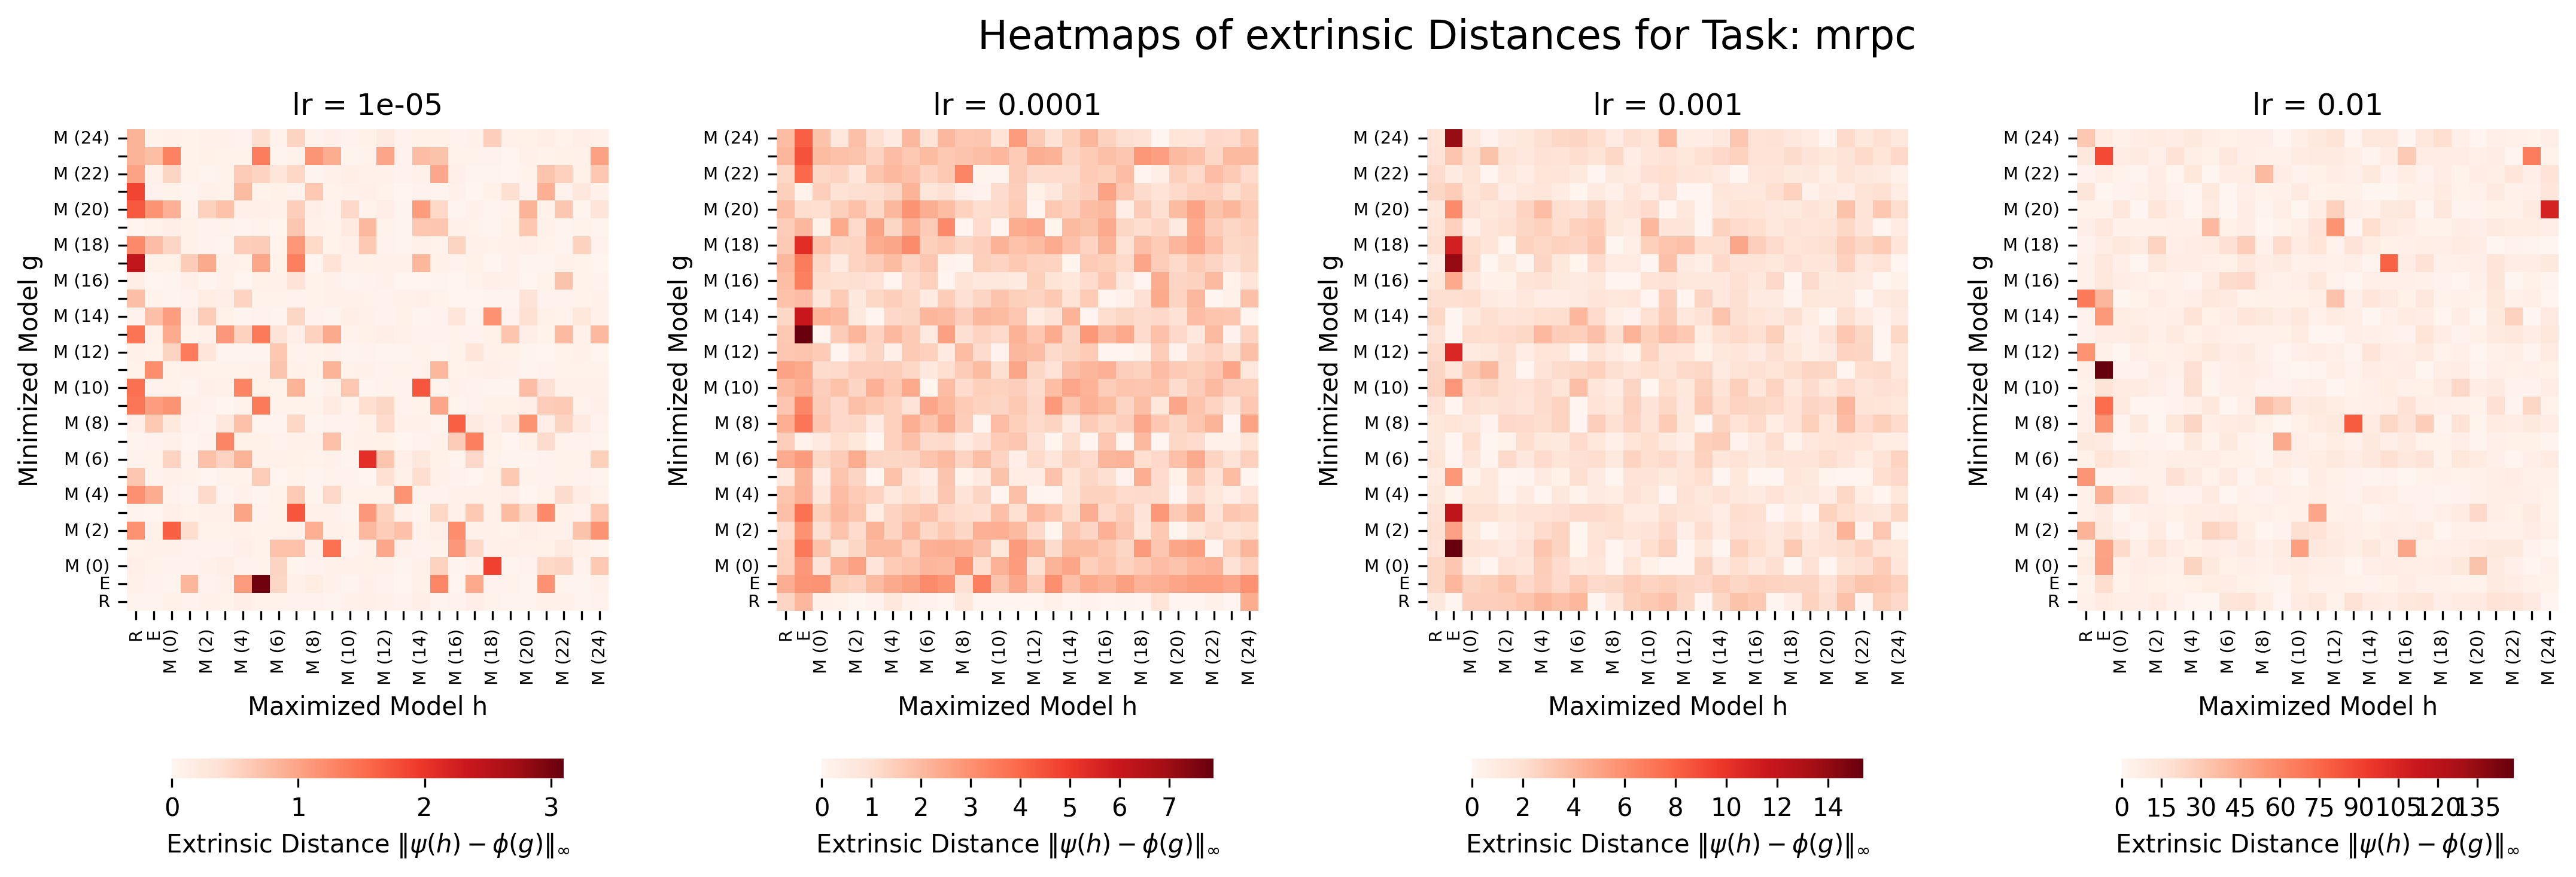
\includegraphics[width=\linewidth]{Abschlussarbeit/Pictures/heatmaps_smaller_circles/Heatmap_extrinsic_distance_all_lrs_mrpc_homotopy.png}
    \caption{Heatmap of extrinsic nonlinear models on \texttt{MRPC} across learning rates.}
    \label{fig:nonlin_intrinsic_model_mrpc}
\end{figure}

\begin{figure}[H]
    \centering
    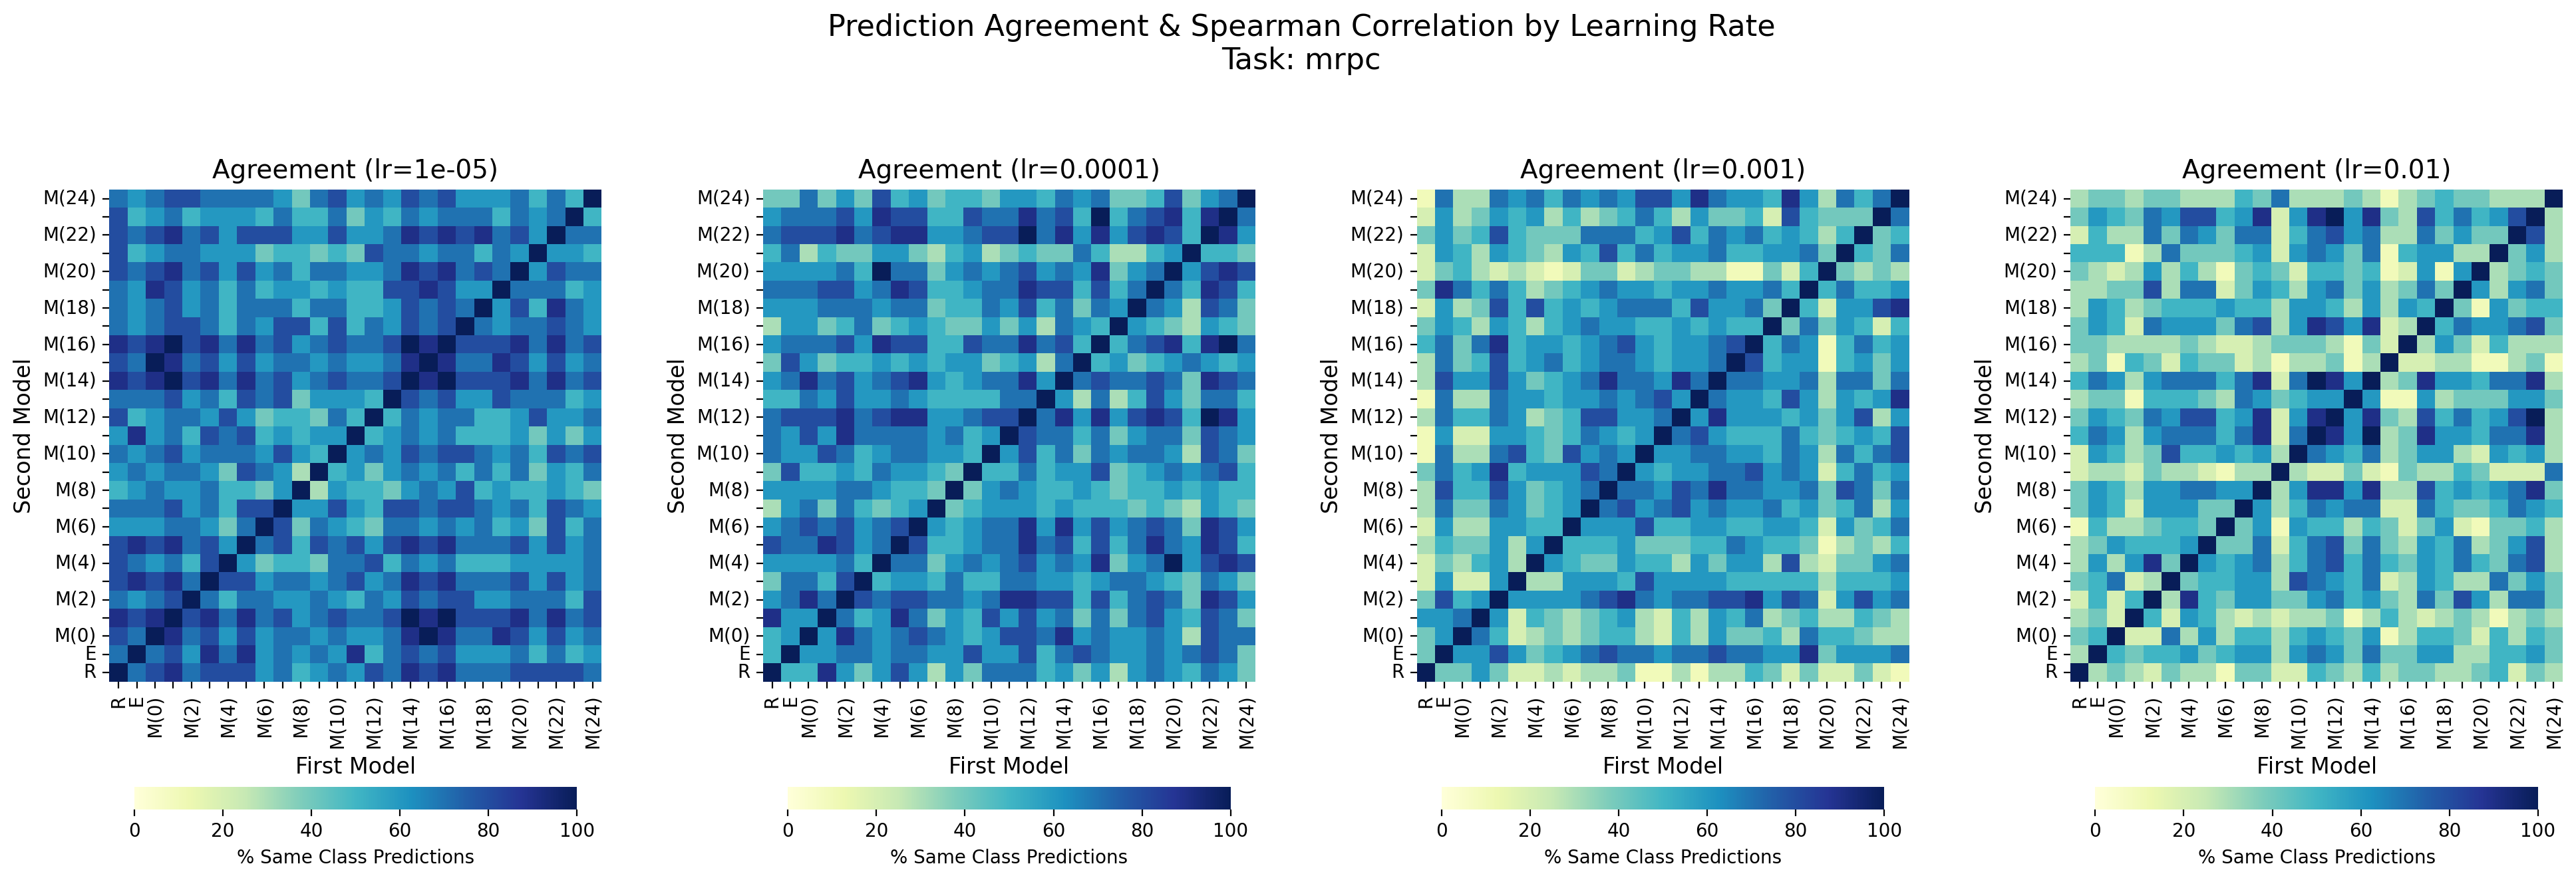
\includegraphics[width=\linewidth]{Abschlussarbeit/Pictures/PredictionAgreement_Spearman/_3Relu_final_training_HeatMap_mrpc_subplots_per_lr_4.png}
    \caption{Heatmap of performance based models on \texttt{MRPC} across learning rates}
    \label{fig:nonlin_performance_model_mrpc}
\end{figure}
Figure~\ref{fig:nonlin_performance_model_mrpc} shows the prediction agreement between all model pairs on the MRPC benchmark, while Figure~\ref{fig:nonlin_intrinsic_model_mrpc} visualizes the corresponding extrinsic homotopy distances.\\
\\
At moderate learning rates (e.g., \( \text{lr} = 10^{-3} \)), we observe both high agreement and low extrinsic distances, indicating functional similarity among models that generalize similarly.  
In contrast, at very low or high learning rates, prediction agreement becomes less structured, and extrinsic distances increase, suggesting instability in training or divergent representational behavior.

Interestingly, even in cases with low agreement, extrinsic distances may remain small, which reflects the power of non-linear transformations to align models that produce dissimilar predictions.

Finally, the asymmetry in the distance maps reflects the directional nature of the extrinsic distance definition, where model \( h \) is approximated via transformations of model \( g \), but not necessarily vice versa.

We now turn to the analysis of extrinsic homotopy and performance-based similarity on the \texttt{SST-2} task. 
Figure~\ref{fig:extr_sst2} shows heatmaps of extrinsic distances across different learning rates, and Figure~\ref{fig:perf_sst2} displays the corresponding prediction agreement and Spearman correlation matrices.

\begin{figure}[h]
    \centering
    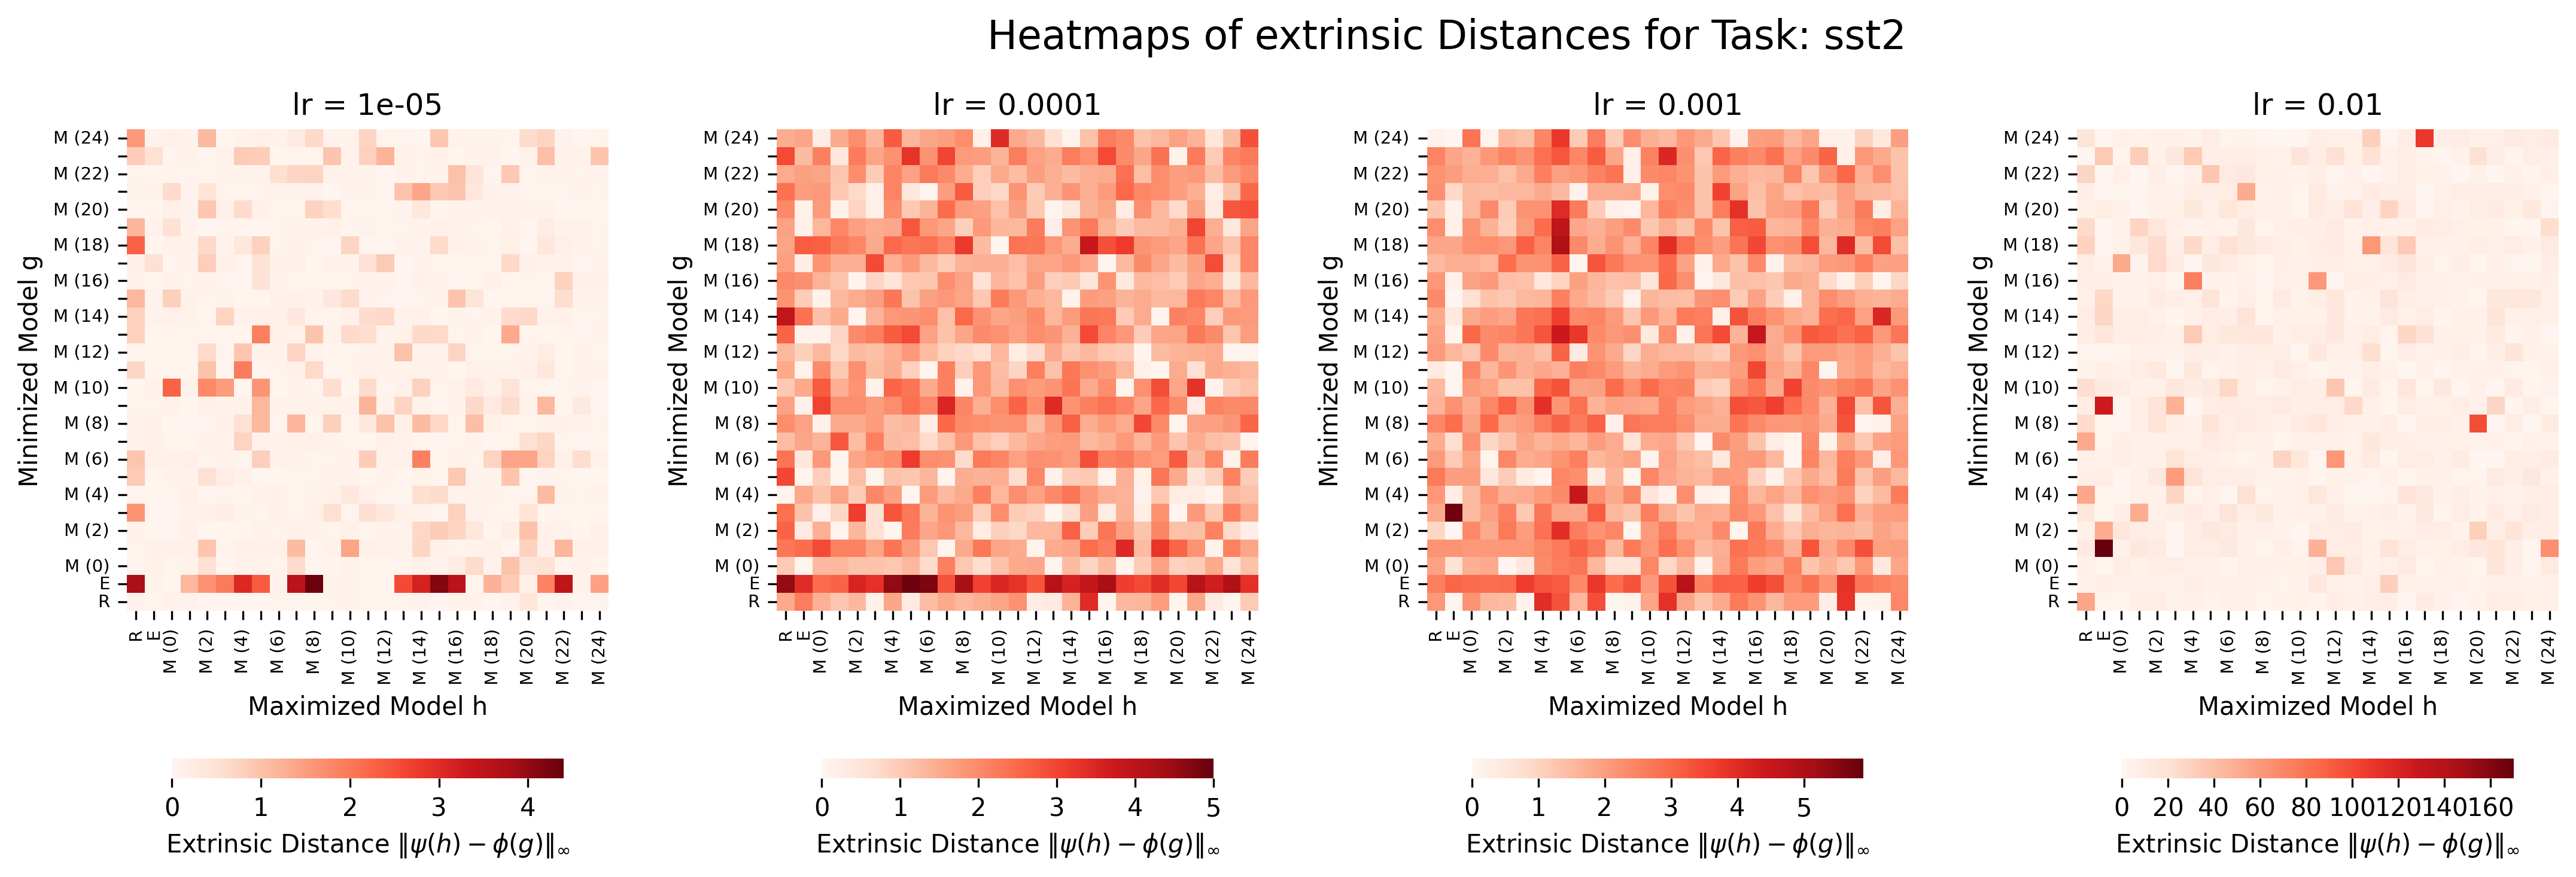
\includegraphics[width=\linewidth]{Abschlussarbeit/Pictures/heatmaps_smaller_circles/Heatmap_extrinsic_distance_all_lrs_sst2_homotopy.png}
    \caption{Heatmaps of extrinsic nonlinear distances on \texttt{SST-2} across different learning rates.}
    \label{fig:extr_sst2}
\end{figure}

\begin{figure}[h]
    \centering
    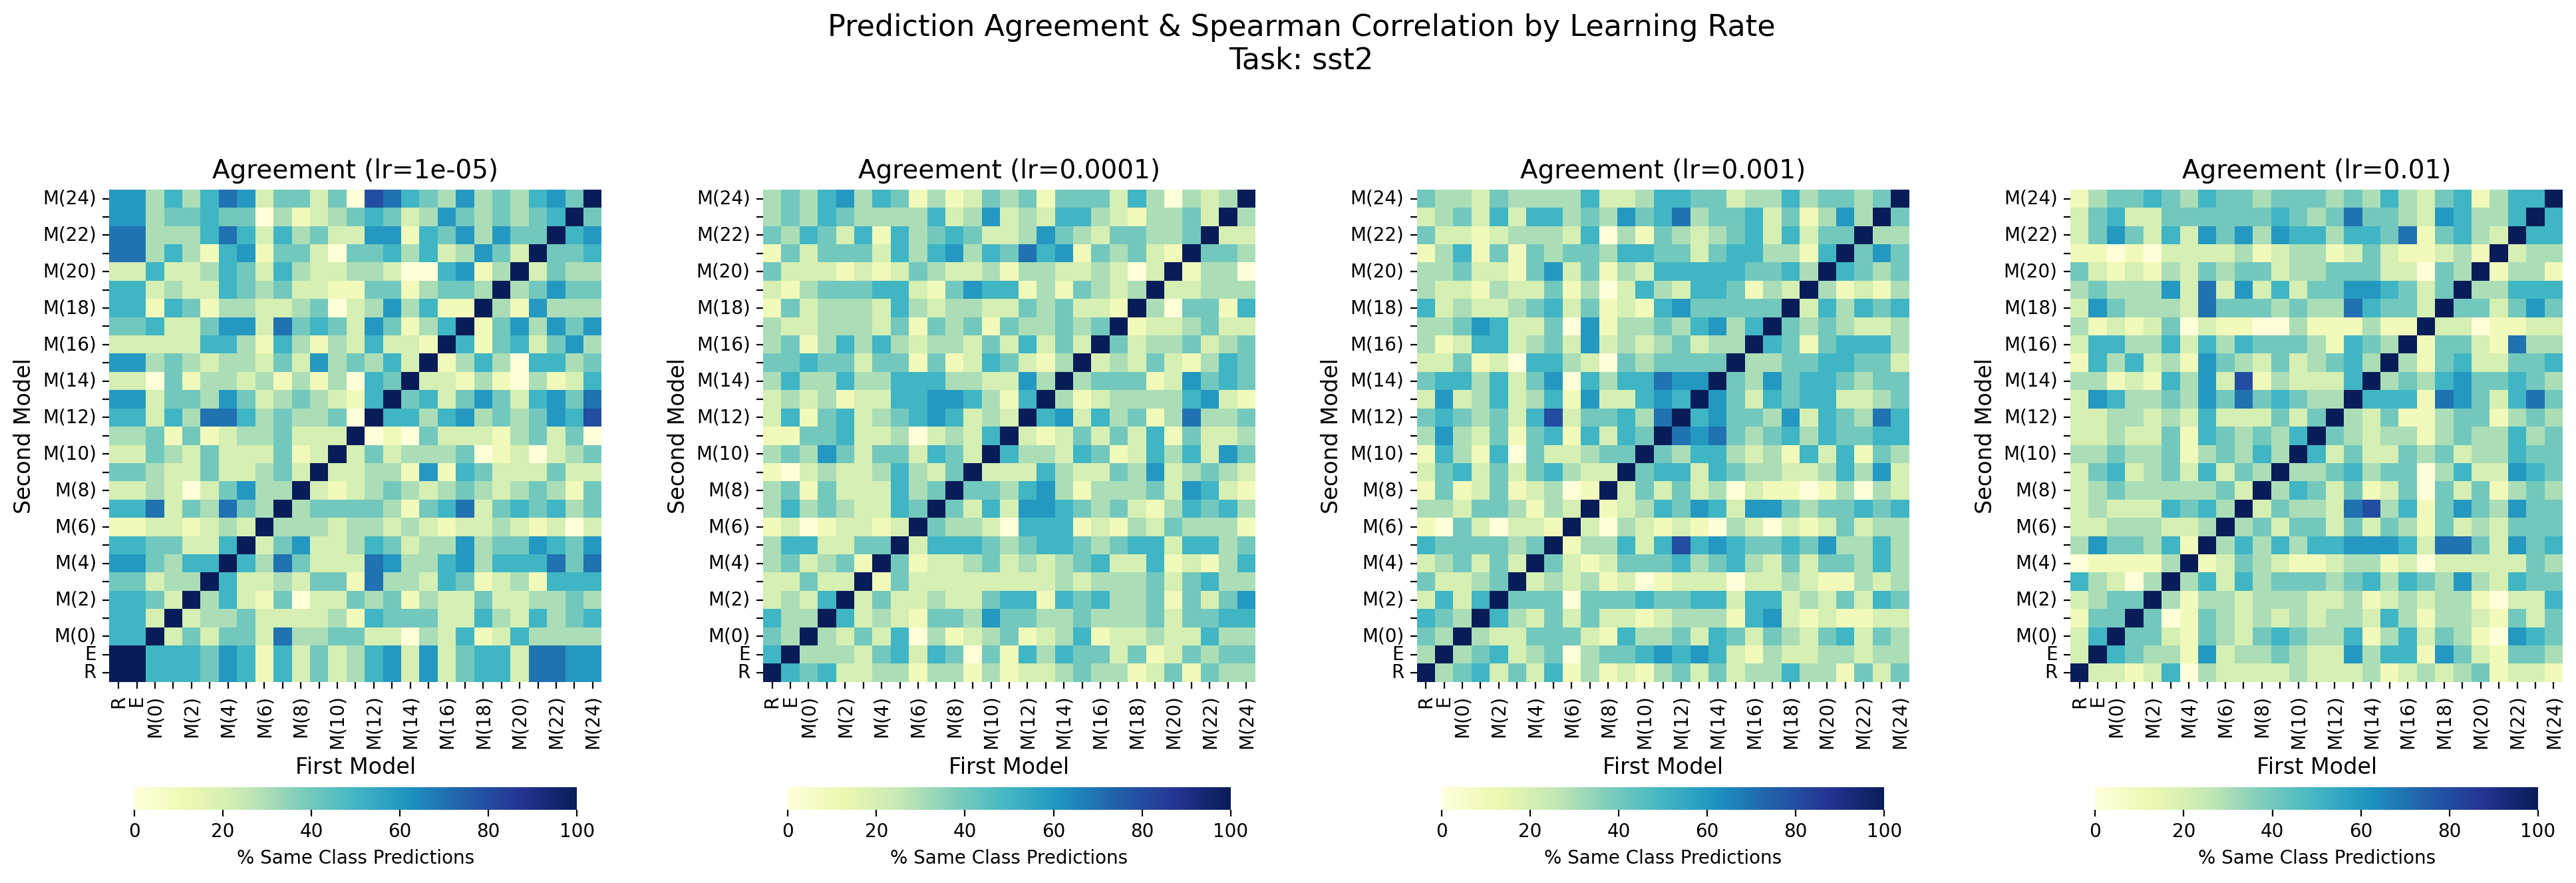
\includegraphics[width=\linewidth]{Abschlussarbeit/Pictures/PredictionAgreement_Spearman/_3Relu_final_training_HeatMap_sst2_subplots_per_lr_4.png}
    \caption{Heatmaps of performance-based similarity (agreement and Spearman correlation) on \texttt{SST-2} across learning rates.}
    \label{fig:perf_sst2}
\end{figure}

Figure~\ref{fig:extr_sst2} shows the extrinsic homotopy distances across different learning rates for the \texttt{SST-2} task, while Figure~\ref{fig:perf_sst2} presents the corresponding prediction agreement between all model pairs.

At a very low learning rate (\( \text{lr} = 1\mathrm{e}{-5} \)), extrinsic distances are generally low, and most model pairs can be aligned well via non-linear transformations, despite relatively low prediction agreement.  
For \( \text{lr} = 1\mathrm{e}{-4} \) and \( \text{lr} = 1\mathrm{e}{-3} \), the distances remain within a narrow and stable range (approximately $0-5$), indicating that the learned representations across models are structurally compatible and can be effectively reconciled, even if their predictions differ.

Compared to \texttt{MRPC}, where extrinsic distances often exceed 10, \texttt{SST-2} exhibits a more consistent representational geometry across the model family.  
This suggests that fine-tuning on\texttt{SST-2} induces less divergent changes in the encoder space and facilitates alignment under non-linear transformations.

At a higher learning rate (\( \text{lr} = 1\mathrm{e}{-2} \)), we again observe a degradation in prediction agreement, and while some extrinsic distances remain low, the overall structure becomes noisier and less interpretable.

We now analyze the \texttt{CoLA} task with respect to extrinsic homotopy and performance-based similarity.  
Figure~\ref{fig:extr_cola} shows the extrinsic distances, while Figure~\ref{fig:perf_cola} presents the corresponding prediction agreement between model pairs.

\begin{figure}[h]
    \centering
    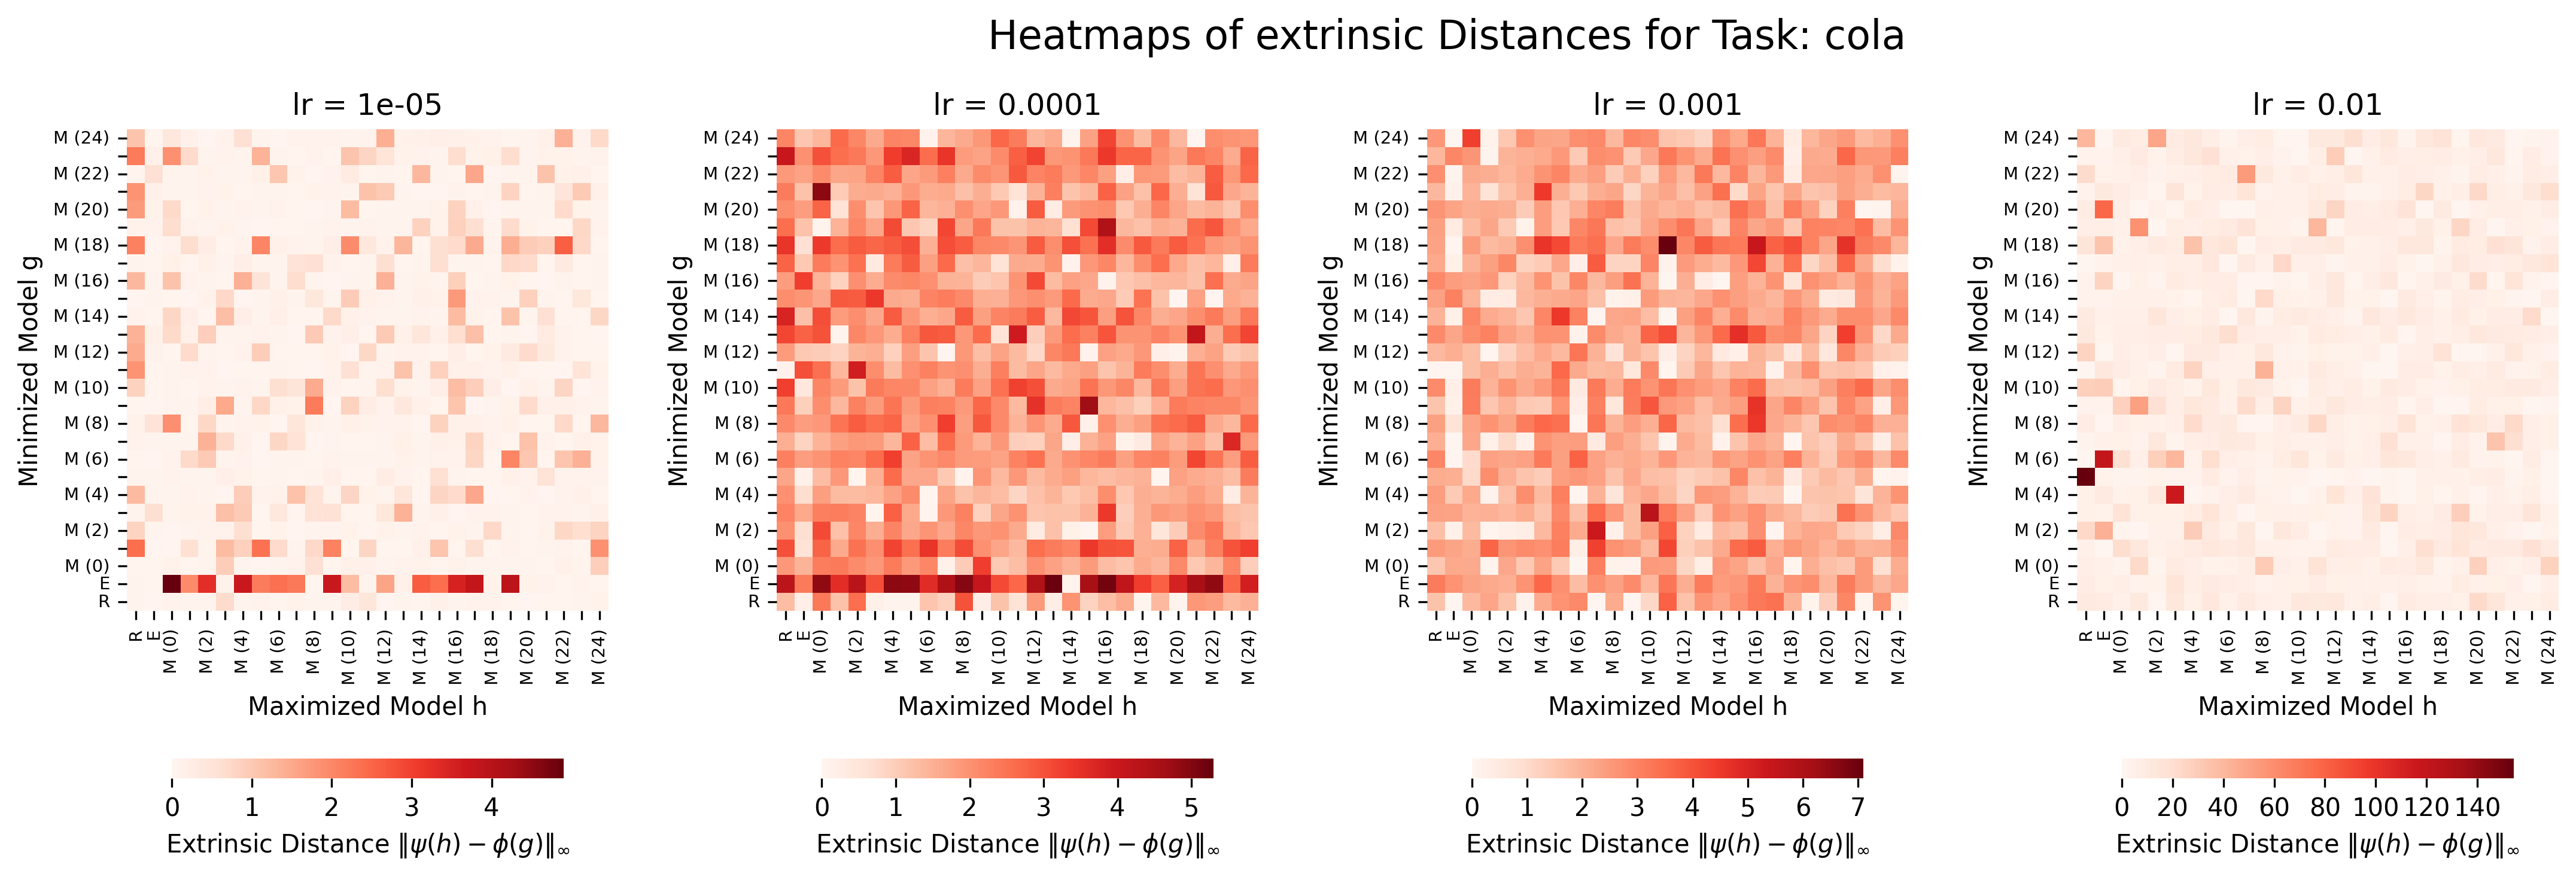
\includegraphics[width=\linewidth]{Abschlussarbeit/Pictures/heatmaps_smaller_circles/Heatmap_extrinsic_distance_all_lrs_cola_homotopy.png}
    \caption{Heatmaps of extrinsic nonlinear distances on \texttt{CoLA} across different learning rates.}
    \label{fig:extr_cola}
\end{figure}

\begin{figure}[h]
    \centering
    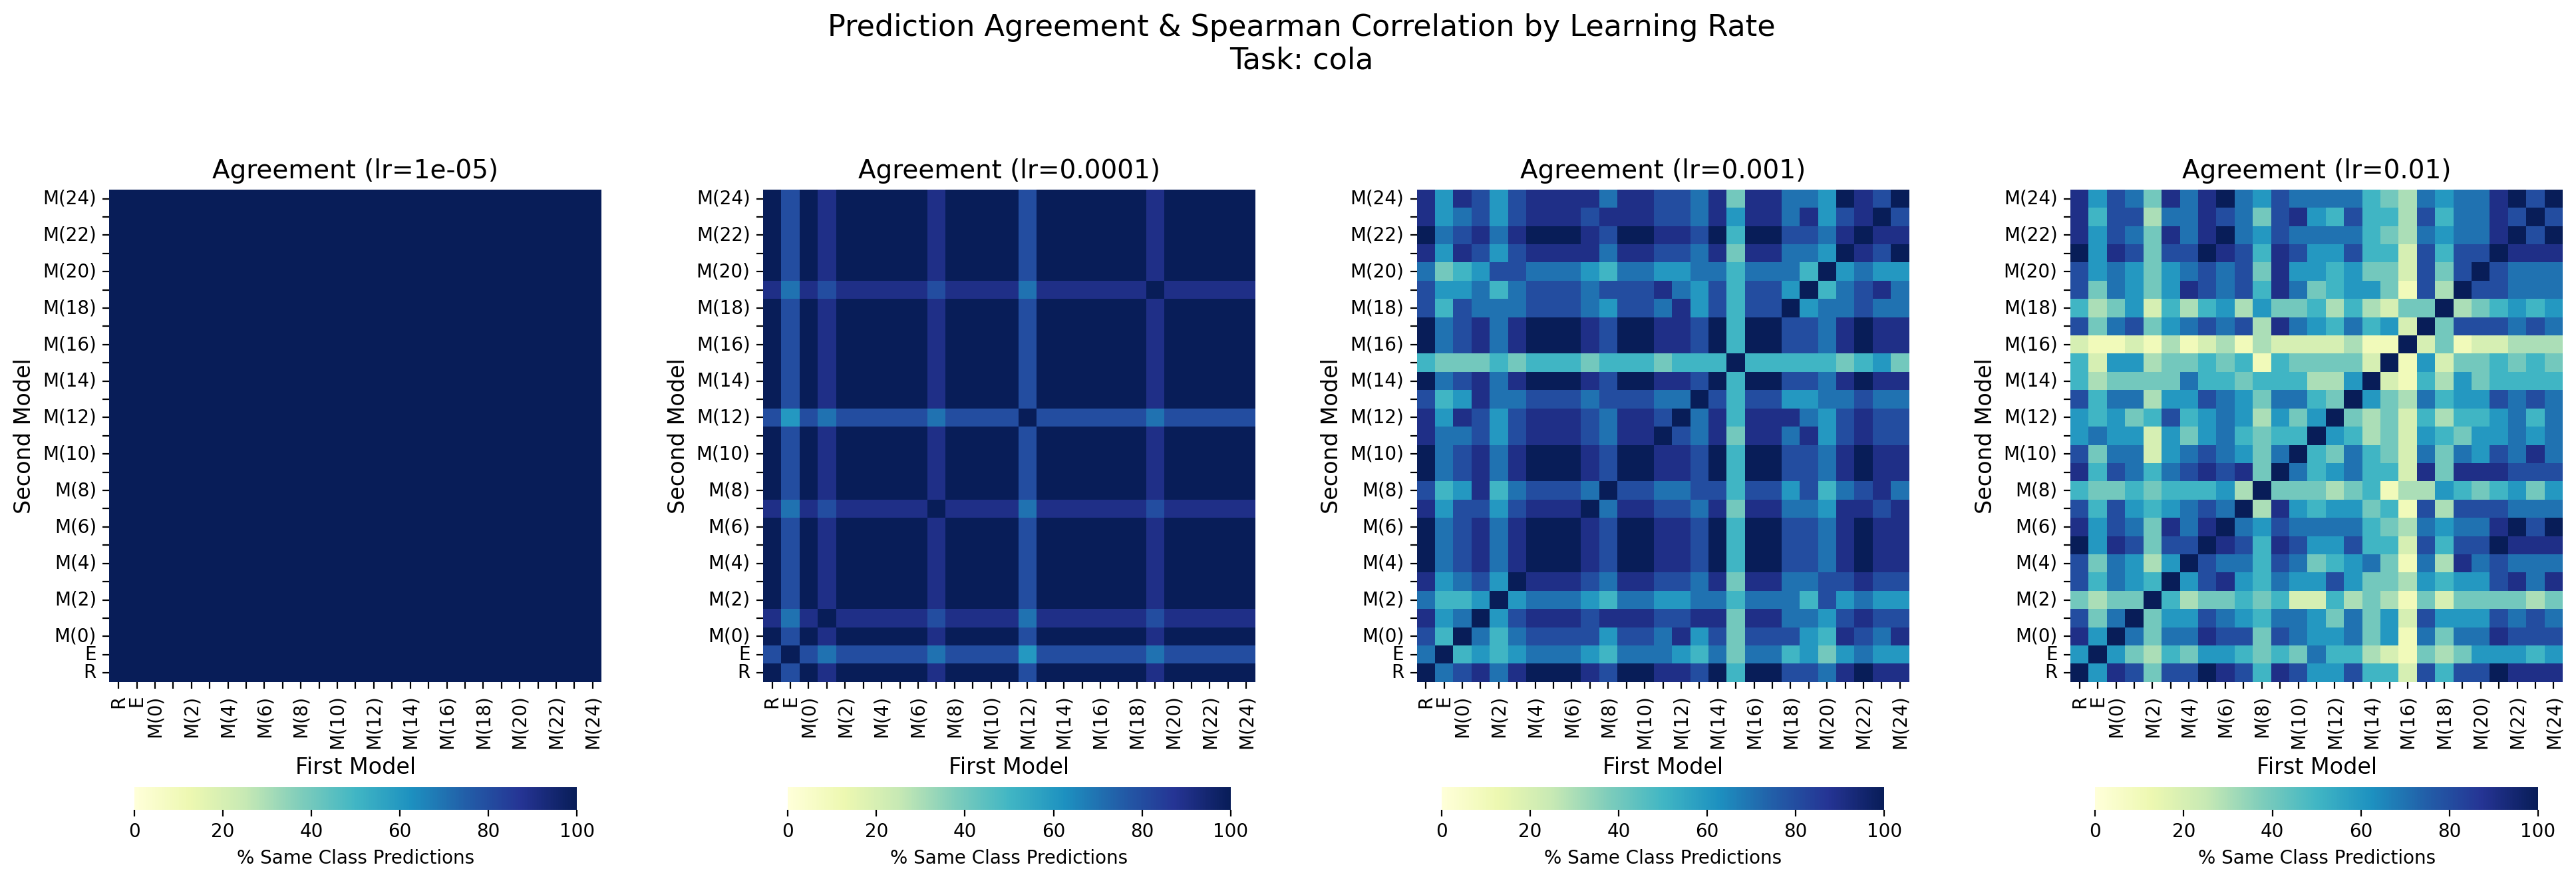
\includegraphics[width=\linewidth]{Abschlussarbeit/Pictures/PredictionAgreement_Spearman/_3Relu_final_training_HeatMap_cola_subplots_per_lr_4.png}
    \caption{Heatmaps of performance-based similarity (agreement and Spearman correlation) on \texttt{CoLA} across learning rates.}
    \label{fig:perf_cola}
\end{figure}

For the \texttt{CoLA} task, we observe a distinct behavior compared to other benchmarks.  
At the lowest learning rate (\( \text{lr} = 1\mathrm{e}{-5} \)), almost all model pairs achieve near-perfect prediction agreement, and the corresponding extrinsic distances remain low.  
This suggests that the models are undertrained and likely converge to trivial classifiers, which is consistent with known difficulties on \texttt{CoLA} due to class imbalance.

As the learning rate increases, model predictions begin to diverge, and prediction agreement decreases.  
At \( \text{lr} = 1\mathrm{e}{-3} \), the agreement heatmaps show unstructured variation, and extrinsic distances rise accordingly—indicating growing representational and functional dissimilarity.

At the highest learning rate (\( \text{lr} = 1\mathrm{e}{-2} \)), prediction agreement becomes highly inconsistent, and individual model pairs exhibit extreme extrinsic distances (up to 140), highlighting training instability.  
Overall, the results illustrate that extrinsic homotopy is highly sensitive to training dynamics and reveals instability that is not always visible through accuracy-based metrics alone.

Finally, we again observe that the extrinsic homotopy matrix is asymmetric.
This aligns with the theoretical foundations of extrinsic homotopy, confirming that the relation is directional and cannot be inferred from symmetric similarity metrics such as agreement or correlation.

